\documentclass[tikz]{standalone}
\usepackage{amsmath}
\usepackage{pgfplots}
\usepackage{csvsimple}

\usetikzlibrary{arrows,intersections,math}

\begin{document}
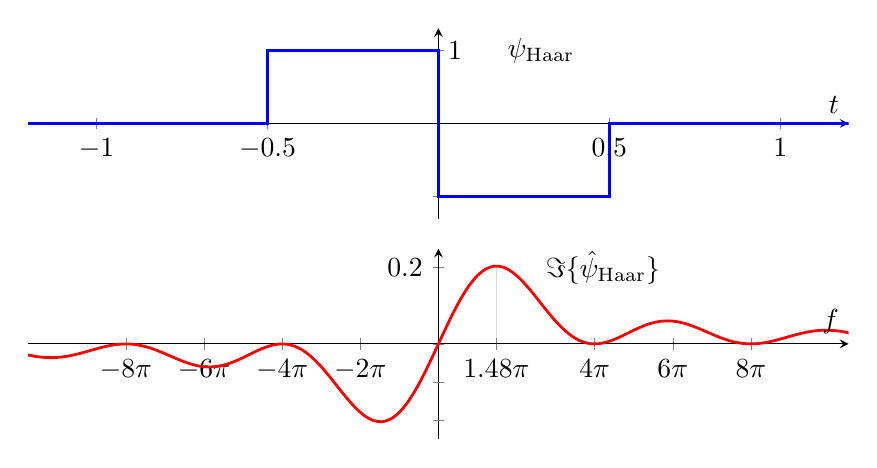
\begin{tikzpicture}
	\begin{scope}[yshift=2.8cm]
		\begin{axis}[width=12cm, height=4cm, xmin=-1.2, xmax=1.2, ymin=-1.3, ymax=1.3,
			axis lines=middle, ytick={-2}, extra y ticks={-1, 1}, extra y tick labels={}, xtick={-1, -0.5, ..., 1.5}]
			\addplot[mark=none, color=blue, line width=1pt] coordinates 
			{(-2, 0 ) (-0.5, 0) (-0.5, 1) (0, 1) (0, -1) (0.5, -1) (0.5, 0) (2, 0)};
			
			\node[anchor=west] at (axis cs: 0, 1) {$1$};
			\node[] at (axis cs: 0.3, 1) {$\psi_{\text{Haar}}$};
			\node[anchor=south east] at (axis cs: 1.2, 0) {$t$};
		\end{axis}
	\end{scope}
	\begin{scope}
		\begin{axis}[axis lines=middle, width=12cm, height=4cm,
			xmin={-10.5*pi}, xmax={10.5*pi}, ymin=-0.25, ymax=0.25,
			y label style={at={(axis cs:{2.5*pi}, 0.2)},anchor=west},
			xlabel=$f$,ylabel=$\Im\lbrace\hat\psi_{\text{Haar}}\rbrace$,
			xtick={-8*pi, -6*pi, -4*pi, -2*pi, 0, 0.742*2*pi, 4*pi, 6*pi, 8*pi},
			xticklabels={$-8\pi$, $-6\pi$, $-4\pi$, $-2\pi$, , $1.48\pi$, $4\pi$, $6\pi$, $8\pi$},
			ytick={0.2}, extra y ticks={-0.2, -0.1, 0}, extra y tick labels={}]
			\addplot[domain=-11*pi:11*pi, samples=100, smooth, color=red, line width=1pt] (\x, {1/(2*sqrt(pi)) * (1 - cos(deg(\x)/2)) / (\x/2)});
			\addplot[color=gray, opacity=0.3] coordinates {({0.742*2*pi}, 0) ({0.742*2*pi}, 0.2041)};
		\end{axis}
	\end{scope}

\end{tikzpicture}
\end{document}
